\begin{figure}[t]
    \centering
    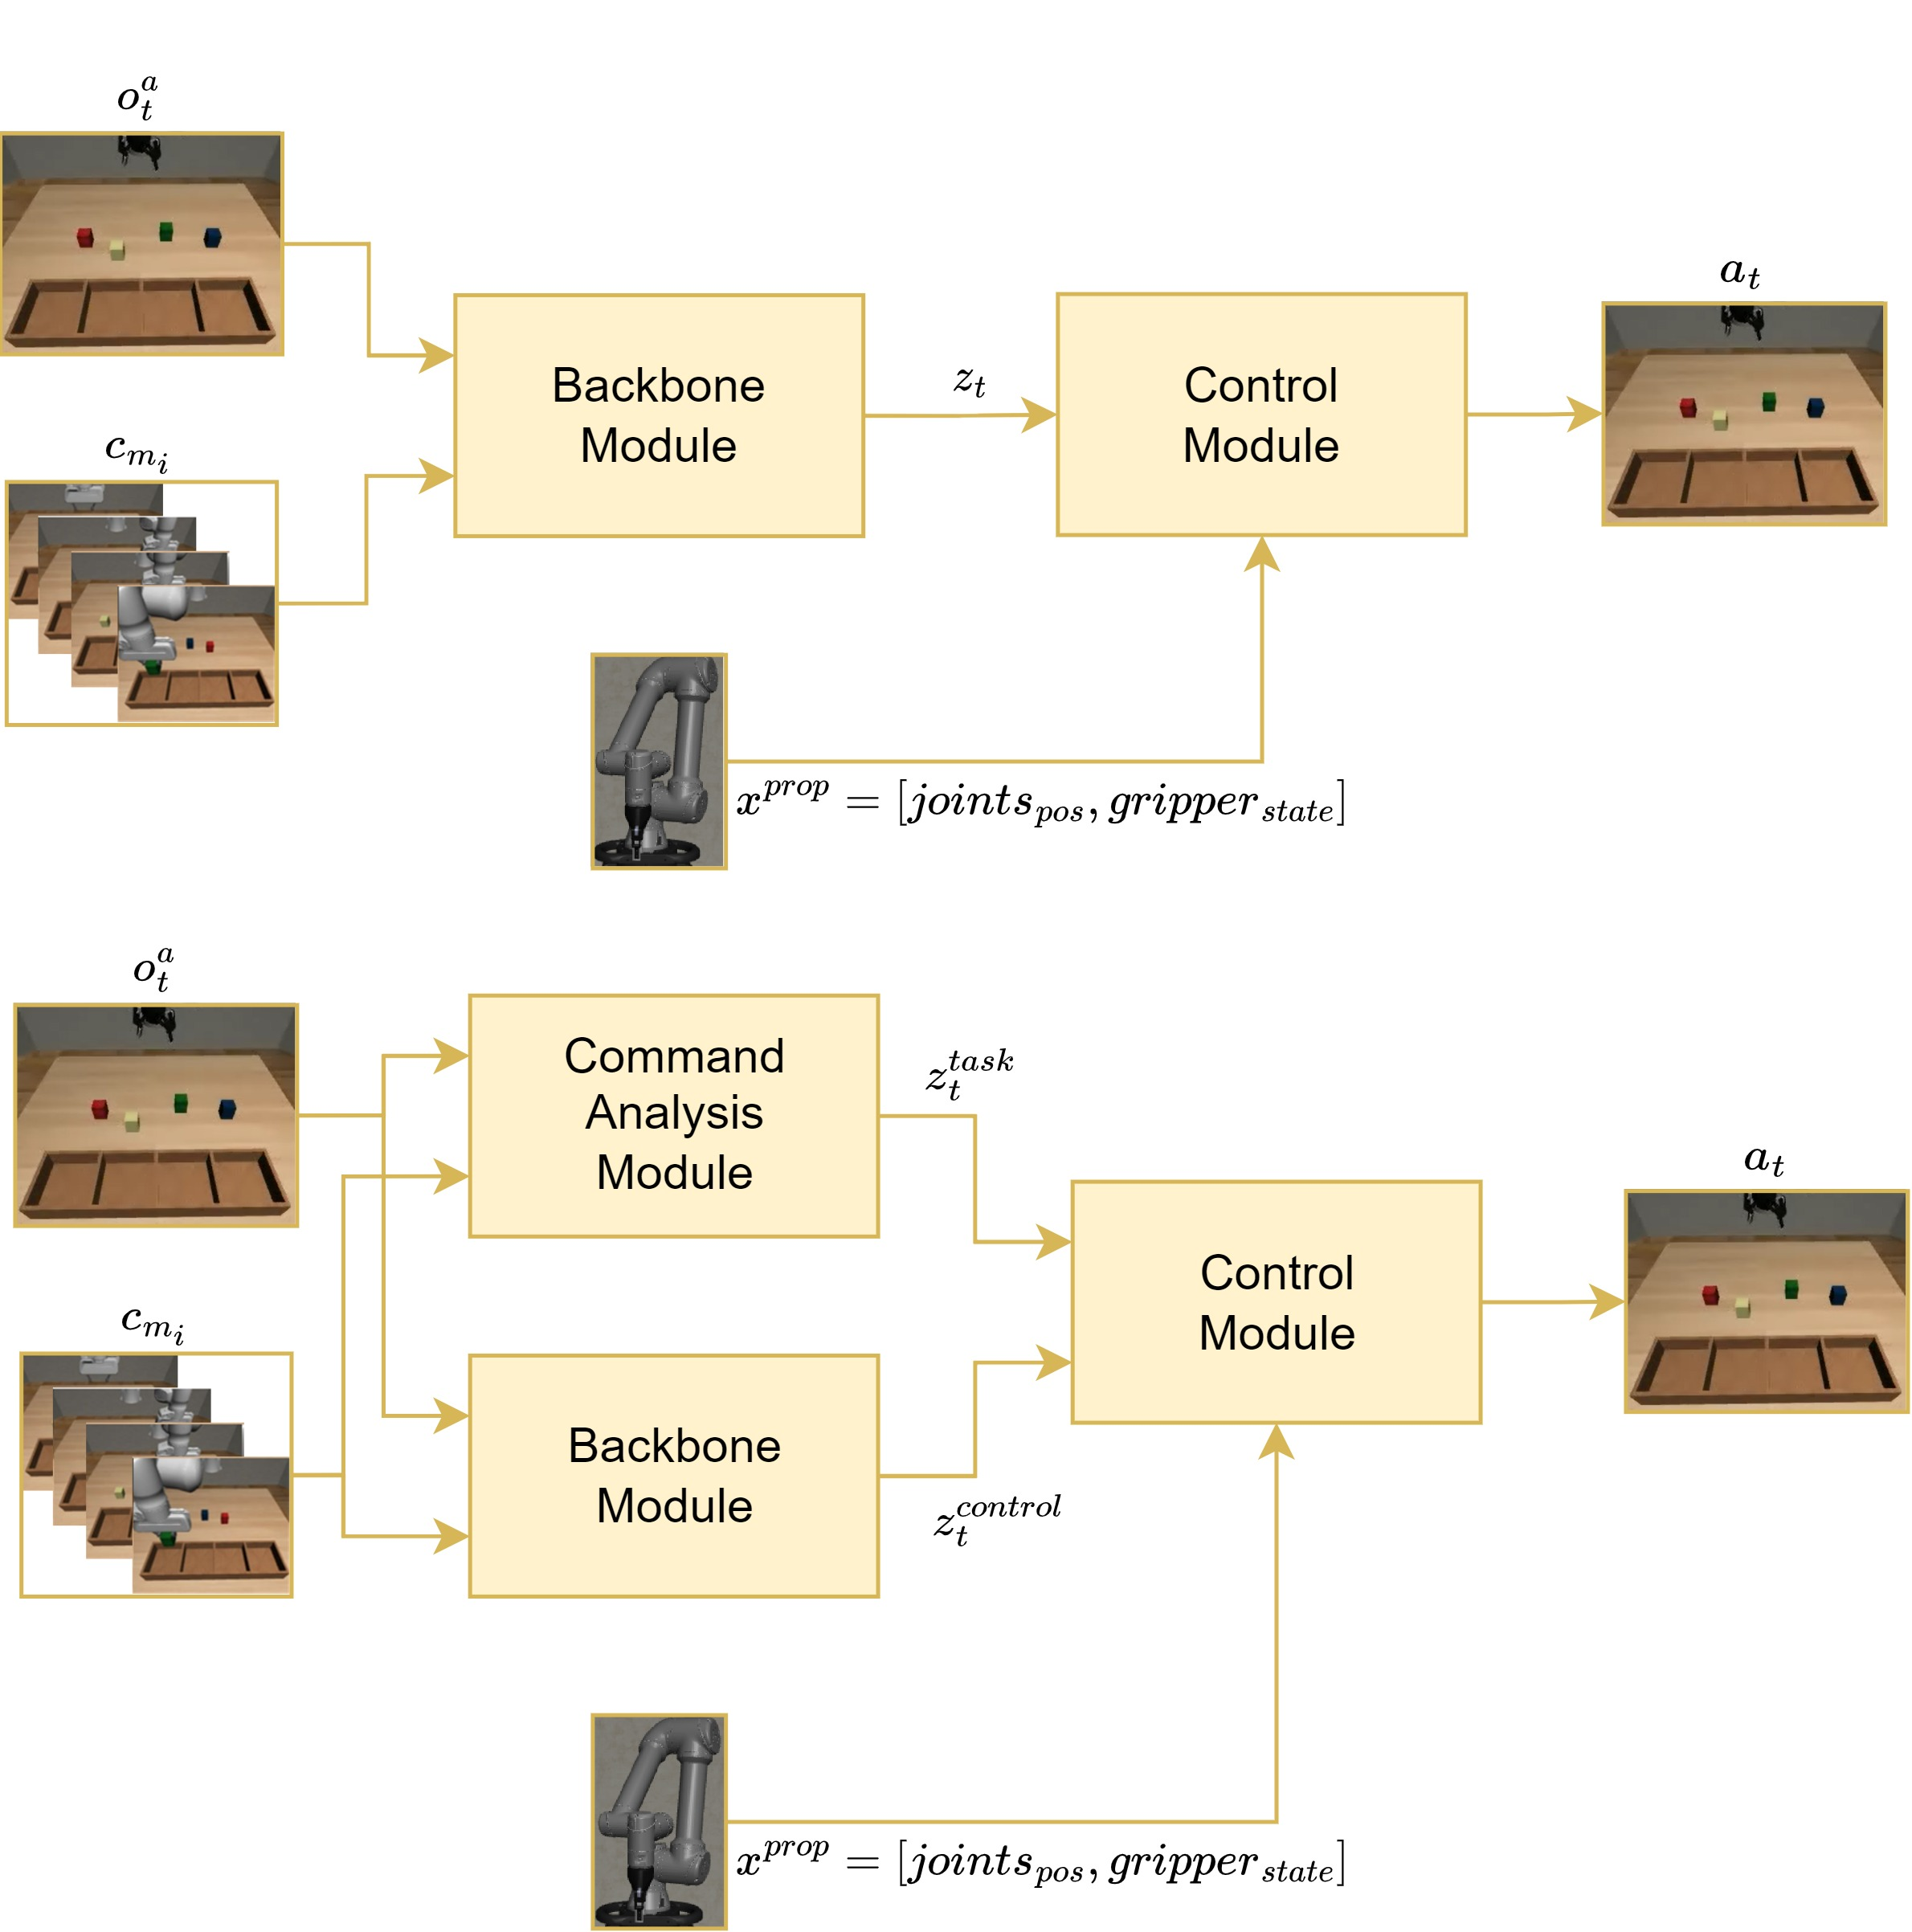
\includegraphics[width=0.7\textwidth]{figures/images/ch3/end_to_end_vs_modular_proprioceptive.jpg}
    \caption{Proprioceptive information is integrated in both the end-to-end architecture (top) and the modular architecture (bottom). The proprioceptive vector, $x^{prop}$, is constructed from the robot's six continuous joint positions and the binary gripper state.}
    \label{fig:end_to_end_vs_modular_proprioceptive}
\end{figure}
